\documentclass{article}
\usepackage[utf8]{inputenc}
\usepackage[T2A]{fontenc} 
\usepackage[serbian]{babel}
\usepackage{amsmath}
\usepackage{amssymb}
\usepackage{mathtools}
\usepackage{amsthm} 
\usepackage{graphicx}
\usepackage{gensymb}
\usepackage[top=27mm, bottom=27mm, left=25mm, right=25mm]{geometry}


\hyphenation{центра-лним пе-ри-фе-ријским најинте-ре-сантнијих по-лу-пре-чник ге-о-ме-три-ји}

\usepackage{hyperref} %hiperlinkovi
\hypersetup{
    colorlinks=true, %linkovi u boji
    linktoc=all,     %linkovi ka svim odeljcima
    linkcolor=blue,  %boja linka
}



\addto\captionsserbian{\renewcommand{\figurename}{Слика}}
\addto\captionsserbian{\renewcommand{\contentsname}{Садржај}}
\addto\captionsserbian{\renewcommand{\refname}{Литература}}
\addto\captionsserbian{\renewcommand{\proofname}{Доказ}}
\newtheorem{theorem}{Теорема}[section]
\newtheorem{definition}{Дефинција}[section]
\newtheorem{stav}{Став}[section]
\newtheorem{tvrdjenje}{Тврђење}[section]
\newtheorem{example}{\sc Пример}
\newtheorem{posledica}{Последица}
\newtheorem{resenje}{Решење}
\newtheorem{lema}{Lema}
\newtheorem{dokaz}{Dokaz}
\newcommand{\Lat}{\fontencoding{OT1}\selectfont}
\newcommand{\minusbinomial}[3][2]{(#2 - #3)^#1}

\begin{document}
\begin{titlepage}
\begin{center}
\Large{Математички факултет}\\
\Large{Универзитет у Београду}
\end{center}
\vspace{1cm}

\begin{center}
\Large{Семинарски рад из предмета Методологија истраживања у настави математике}
\end{center}

\begin{center}
\Huge{\textbf{Круг}
\end{center}

\vspace{2cm}
\begin{figure}[h!]
        \centering
        \includegraphics
        [width = 0.4\textwidth]
        {matf.png}
\end{figure}


\vspace{2cm}

\begin{flushright}
Студент:
Милена Дуканац 1020/2017\\
\end{flushright}

\vfill

\begin{center}
Београд,\\
август 2018.
\end{center}

\end{titlepage}

\thispagestyle{empty}

\tableofcontents

\newpage
\pagenumbering{arabic}

\section{Увод}

Rekonstrukcija genoma kroz sekvenciranje DNK je važan problem u genomici. Ovaj problem izgleda jednostavno, ako se genom može čitati base-by-base od 5' ka 3'. Nažalost, postojeće biotehnologije ne mogu proći kroz ceo hromozom, jer je predugačak. Umesto toga, rekonstruišemo genom indirektno. Prvo, genom se razija na fragmente koristeći pristup čitanja celog sekvencioniranog genoma (whole genome shotgun approach); zatim mašina za sekvencioniranje dekodira DNA sekvence na osnovu ovih fragmenata. Ove DNA sekvence se nazivaju čitanja (reads). Zbog slučajnog uzorkovanja, ekstahovana čitanja pokrivaju ceo genom uniformno. Lepljenjem ovih čitanja u jedno možemo računski rekonstruisati genom. Ovaj proces je poznat kao de novo genomsko asembliranje.\\

Sanger sekvenciranje je bila najranija tehnika sekvenciranja. Dva asemblera su bila razvijena za sastavljanje čitanja Sanger sekvenciranja. Oni su OLC asembler Celera i De Brujinov grafički asembler Ojlera. Naš čovečiji referentni genom sastavljen je korišćenjem ova 2 pristupa. Međutim, kako je Sanger sekvenciranje niskopropusno i skupo, samo nekoliko genoma je sasatvljeno Sanger sekvenciranjem.\\

Porast sekvenciranja druge generacije promenio je igru. Možemo sekvencirati stotine miliona čitanja efikasno i isplativo. Međutim, sekvenciranje čitanja druge generacije je kratko. Neki po narudzbini napravljeni genomski asembleri su razvojeni za rekonstrukciju genama na osnovu kratkih čitanja. Njihov uspeh  je doveo do većeg broja uspešnih de novo asemblerskih projekata, uljučujući rekonstrukciju genoma Dzima Votsona i panda genoma. Iako je ovaj pristup ekonomičan, on obično daje fragmentisane genome, jer su čitanja kratka i područja koja se ponavljaju su duga.\\

Nedavno je na raspolaganju sekvenciranje treće generacije, koje može sekvencirati duga čitanja (dužine oko 10000 bp). Iako duga čitanja mogu rešiti redosled ponavljajućih regiona, ona imaju visoku stopu greške (15\%-18\%). Razvijen je veliki broj računskih metoda za ispravljanje grešaka sekvenciranja čitanja treće generacije.\\

\section{Čitanje celog sekvencioniranog genoma}

Da bi se sastavio genom, prvi korak je sekvenciranje skupa čitanja na osnovu uzorka genoma. Za ovu svrhu postoje 2 protokola: (1) sekvenciranje celog genoma i (2) sekvenciranje matičnih parova. U nastavku će oni biti ukratko opisani.

\subsection{Sekvenciranje celog genoma}

Sekvenciranje celog genoma ukljucuje 3 koraka koja su prikazana na slici 2.1.\\

Prvo, uzorak genoma se na slučajan način razbija na DNA fragmente pomoću sonication ili enzimskog sečenja; zatim korak odabira veličine ekstrahuje DNA fragmente određene fiksirane dužine (veličina umetka). Na kraju se vrši single-end ili paired-end sekvenciranje DNA fragmenata. Za single-end sekvenciranje, sekvencer čita jedan kraj svakog DNA fragmenta. Za paired-end sekvenciranje, sekvencer čita oba kraja DNK fragmenta. (Sekvenceri treće generacije čitaju čitav DNA fragment. Mi to smatramo single-end čitanjem.) Slika 2.2 daje jedan primer. Za single-end sekvenciranje, dobijamo čitanje sa 5' kraja lanca DNA fragmenta, tj. ACTCAGCACCTTACGGCGTGCATCA. Za paired-end sekvenciranje, dobijamo 5' čitanja i forward i reverse templates DNA fragmenta (u unutrašnjoj orijentaciji, tj. čitanje šablona od 5' ka 3'), tj.

\begin{itemize}
    \item {ACTCAGCACCTTACGGCGTGCATCA}
    \item {AGTTTGTACTGCCGTTCAGAACGTA}
\end{itemize}

Drugo čitanje je inverzni komplement prvog, jer se ono dobija iz obrnutog šablona.\\

Za asembliranje genoma, veličina umetka (dužina DNK fragmenta) je veoma važan parametar. Različite tehnologije sekvenciranja imaju različita ograničenja za veličinu umetka. Na primer, Illumina Hi-sek može izvršiti samo paired-end sekvenciranje za DNK fragmente veličine umetaka $< 1000$ bp. Za treću generaciju sekvenciranja, granica veličine umetka može biti veća od 10000 bp.\\

%Slika 2.1 i opis Figure 5.1 iz knjige
%Slika 2.2 i opis Figure 5.2 iz knjige
%Slika 2.3 i opis Figure 5.3 iz knjige

\subsection{Mate-pair sekvenciranje (sekvenciranje matičnih parova)}

Sekvenceri druge generacije mogu izvući pair-end čitanja sa oba kraja kratkih DNA fragmenata (veličine umetka manje od 1000 bp). Za izvlačenje pair-end čitanja dugih DNA fragmenata možemo koristiti mate-pair proces sekvenciranja. Slika 2.3 prikazuje mate-pair proces sekvenciranja.  Prvo, dugi DNA fragmenti neke fiksirane veličine umetka (npr. 10000 bp) se bira sečenjem gena. Zatim se dugi fragmenti cirkularizuju pomoću adaptora. Cirkularizovani DNA-ovi su fragmentisani i samo se zadržavaju fragmenti koji sadrže adaptore (say, by biotin pull-down). Na kraju, pomoću pair-end sekvenciranja, pair-end čitanja se sekvenciraju na osnovu DNA fragmenata sa adaptorima.\\

Orijentacija pair-end čitanja pročitanog od strane mate-pair sekvencera se razlikuje od onog koji je pročitan od strane pair-end sekvencera. Mate-pair sekvenceri daju dva čitanja sa oba kraja svakog DNA fragmenta u spoljašnjoj orijentaciji umesto u unutrašnjoj orijentaciji. Npr. za Dna fragment na slici 2.2 mate-pair sekvenciranje će dati:
\begin{itemize}
    \item {TGATGCACGCCGTAAGGTGCTGAGT}
    \item {TACGTTCTGAACGGCAGTACAAACT}
\end{itemize}

Iako protokol za mate-pair sekvenciranje može izvući pair-end čitanja sa velikom veličinom umetka, on zahteva veći broj ulaznih DNK-a za pripremu sekvencerskih biblioteka i sklon je lažnim greškama.

\subsection{De novo sekvenciranje genoma za kratka čitanja}

Druga generacija sekvenciranja nam omogućava da dobijemo skup single-end ili paired-end kratkih čitanja za ceo genom. De novo asembliranje ima za cilj da preklopi čitanja koja se dobijaju u ispravnom redosledu i da rekonstuiše genom.\\

% Figure 5.4 i slika 2.4

Problem asembliranja genoma je računski težak. Čak i kada ne postoji greška sekvenciranja, ovaj problem je ekvivalentan suprstring problemu za koji se zna da je NP-kompletan. (Problem superstringa - na osnovu skupa stringova S, težimo da nadjemo superstring, najkraći string P takav da je svaki string s iz skupa S podstring stringa P. Na primer, ako je $S = \{ACATGC, ATGCGTGT, GTGTACGT\}$, onda je superstring ACATGCGTGTACGT.) \\

Mnogi de novo asembleri predlažu da se sastavljaju kratka čitanja. Opšte rešenje uključuje 4 koraka kao što je prikazano na slici 2.4. U prvom koraku se ispravljaju greške sekvenciranja u čitanju. Na osnovu korigovanih čitanja, u drugom koraku se vrši lepljenje čitanja preklapanjem. U idealnom slučaju, želimo da zalepimo sva čitanja tako da formiraju kompletan genom. Zbog ponavljanja, postoje dvosmislenosti i ne uspevamo da zalepimo čitanja tako da rekonstruišemo kompletan genom. Postojeći metodi daju skup kontigenata, pri čemu svaki kontigent predstavlja podregion uzorka genoma. Zatim, koristeći pair-end čitanja, pokušavamo da rekonstruišemo redosled kontigenata tako da formiramo skelet.(Svaki skelet je niz kontigenata. Jos se naziva i superkontig ili metakontig.) Na kraju, čitanja se preuređuju na skeletima, tako da se popune praznine između susednih kontigenata.\\

Ovaj odeljak je organizovan na sledećí način. Odeljak 2.3.1. razmatra korekciju grešaka čitanja. Zatim predstavljamo korak izgradnje kontigenata. Grubo govoreći, postoje 2 pristupa za izgradnju kontigenata: (1) prošireni base-by-base pristup i (2) Debrujin graf pristup. Oni će biti pokriveni u sekcijama 2.3.2 i 2.3.3, respektivno. Na kraju, skelet korak i korak popunjavanja praznina su opisani u odeljcima 2.3.4 i 2.3.5.\\

\subsection{Korekcija greški čitanja}

Greške u sekvencerskom čitanju mogu dovesti u zabludu de novo asemblere. Bolje je, ako ih možemo ispraviti pre sastavljanja genoma.\\

Pretpostavimo da se genom uzorkuje sa velikom pokrivenošću. Jednostavna metoda je da se identifikuju i skupe veoma slčna čitanja. Ako čitanje sadrži bazu koja se razlikuje od konsenzus niske, takva baza je greška sekvenciranja.\\

Na primer, razmotrimo sledeći skup čitanja $R = \{R_1 = AAGTGAA, R_2 = AGTGCAG, R_3 = ACTTCAC, R_4 = TGAAGTG\}$. Slika 2.5 pokazuje višestruko sekvenciono poravnanje $R_1, R_2, R_3, R_4$ ($R_3$ je inverzni komplement od $R_3$). Baza C na 5. poziciji $R_2$ je nekonzistentna sa bazom A u ostala tri čitanja. Baza C je verovatno greška sekvenciranja. Kako bismo ispravili grešku, možemo konvertovati bazu C na 5. poziciji u čitanju $R_2$ u bazu A.
%Celo ovo je preskoceno, presla sam na sledecu sekciju

\subsection{Problem spektralnog poravnanja}

Neka je $R = \{R_1, . . . , R_n\}$ skup čitanja koja su sekvencionisana iz uzorka genoma T. Označimo sa $\tau$ k-mere koji se pojavljuju u T. $\tau$ može biti aproksimirano sa $\{t \in S_R $\vert$ t je k-mer koji se pojavljuje najmanje u M čitanja\}$.\\

Čitanje R ćemo označiti kao $\tau$-string, ako je svaki k-mer iz skupa R u T. Kako se $\tau$ sastoji od svih k-mera koji se nalaze u T, za svako čitanje iz uzorka genoma T $\tau$-string. Ako $R[1...m]$ nije $\tau$-string, očekuje se da R ima grešku. Kako bi se ispravila greška od R, predložen je problem spektralnog poravnanja. Problem spektralnog poravnanja ima za cilj da prodnađe minimalni broj ispravki (ubacivanje, brisanje, mutacija) koje transformišu R u $\tau$-string $R'$. Ako postoji jedinstven način da se $R$ ispravi i broj ispravki je najviše $\delta$, onda za $R'$ kažemo da je korigovano čitanje $R$.\\

Za prethodni primer gde je $R = \{R_1 = AAGTGAA, R_2 =
AGTGCAG, R_3 = ACTTCAC, R_4 = TGAAGTG\}$, $\tau$ se može aproksimirati sa $\{t \in S_R $\vert$ t je k-mer koji se pojavljuje u najmanje 2 čitanja\}$.  Tj. $T = \{AAGT, ACTT, AGTG, CACT, CTTC, GAAG, GTGA, TCAC, TGAA, TGCA, TTCA\}$. Primetimo da su $R_1, R_2, R_3$ i $R_4$ $\tau$-stringovi. Stoga se pretpostavlja da su ispravni. Za čitanje $R_2 = AGTGCAG$, $R_2$ nije $\tau$-string, jer k-meri GTGC i GCAG nisu u $\tau$. Kako bismo ispravili $R_2$, možemo uvesti jednu mutaciju $C \rightarrow A$ na poziciji 5 i dobićemo $R'= AGTGAAG$, koji je $\tau$-string. Ako je $\delta = 1$, korekcija je prihvaćena, jer je ovo jedini način da se R pretvori u $\tau$-string pomoću najviše jedne mutacije. \\

Problem spektralnog poravnanja se može rešiti u polinomijalnom vremenu. Kako bismo pojednostavili diskusiju, pretpostavimo da ne postoji idealna greška u prvih k baza od R. Potrebne su nam dve definicije. Prvo, za svaki k-mer t i svaku bazu $b \in \{A, C, G, T\}$ označimo sa $b \cdot t[1...k-1]$ k-mer dobijen nadovezivanjem t sa $t[1...k-1]$. (Na primer, ako je 4-mer GAAG i $b = T$, onda je $b  \cdot t[1..k-1] = TGAA$). Drugo, definišimo $dist(i, t)$ kao minimalno rastojanje između $R[1...i]$ i bilo kog $\tau$-stringa koji se završava na k-meru t. Sledeća lema prikazuje rekurzivnu formulu za $dist(i, t)$\\

\begin{lema}{Označimo sa $\rho(x, y) = 0$, ako je $x = y$, a 1 u suprotnom.}
    \item {Za $i = l$ i $t \in \tau $ (osnovni slučaj), $dist(k, t) = Hamming(R[1..k], t)$}
    \item {Za $i \geq k$ i $t \in \tau $ (rekurzivni slučaj), $$dist(i, t) = \min \begin{cases} 
          $\smash{\displaystyle \min_{b \in \{A, C, G, T\}}} \{ dist(i - 1, b \cdot t[1..k - 1])\} & match \\
          dist(i - 1, t) + 1 & delete \\
           $\smash{\displaystyle \min{\{dist(i, b \cdot t[1..k - 1]) + 1\}}} & insert
       \end{cases}$$ }
\end{itemize}
\end{lema}

%Dokaz preskocen
\newpage
Minimalno edit rastojanje između R i bilo kog $\tau$-stringa je $\smash{\displaystyle \min_{t \in \tau}} dist(\vert R\rvert, t)$.\\

S obzirom na rekurzivnu formulu datu u prethodnoj lemi, prvo što nam pada na pamet jeste da koristimo dinamičko programiranje da izračunamo $dist(\vert R\rvert, t)$ za sve $t \in \tau$, zatim možemo izrаčunati $\smash{\displaystyle \min_{t \in \tau}} dist(\vert R\rvert, t)$. Međutim, ova rekurzivna formula ima ciklične zavisnosti i dinamičko programiranje se ne može koristiti.\\

U nastavku ilustrujemo da ciklična zavisnost može postojati. Prvo definišemo graf zavisnosti G za rekurzivnu formulu $dist(i, t)$. Graf zavisnosti $G(V, E)$ je graf sa skupom verteksa $V = \{v_s\} \bigcup \{(i, t) $\vert$ i = k, ..., \vert R\rvert, t \in \tau\}$. S obzirom na lemu 5.1, za svaki čvor $(i, t)$ (rekurzivni slučaj) gde je $i \geq k$, lema 5.1 implicira da je $dist(i, t)$ minimum između $dist(i - 1, b \cdot t[1..k - 1]) + r (R[i], t[k])$, $dist(i - 1, t) + 1$ i $dist (i, b \cdot t[1..k - 1]) + 1$, gde $b \in \{A, C, G, T\}$. U grafu zavisnosti G kreiramo 3 vrste grana:\\
\begin{itemize}
    \item {match edge: $((i - 1, b \cdot t[1..k - 1]), (i, t))$, čija je težina $\rho (t[k], R[i])$}
    \item {delete edge: $((i - 1, t), (i, t))$, čija je težina 1}
    \item {insert edge $((i, b \cdot t[1..k - 1]), (i, t))$, čija je težina 1}
\end{itemize}

Za svaki čvor $(k, t)$ (osnovni slučaj) $dist(k, t) = Hamming(R[1..k], t)$ i ne zavisi ni od jedne druge vrednosti. Tako da uključujemo granu $(v_s,(k, t))$ težine $Hamming(R[1..k], t)$.\\

Figura 5.6(iz knjige) predstavlja zavisnost grafa od čitanja $R_2 = \{AGTGCAG\}$ i $\tau = \{AAGT, AGTG, GAAG, GTGA, TGAA, TGCA\}$. Na primer, čvor $(6, TGAA)$ zavisi od 3 grane:
\begin{enumerate}
    \item {match grana $((5, GTGA), (6, TGAA)),$}
    \item {delete grana $((5, TGAA), (6, TGAA),$}
    \item {insert grana $((6, GTGA), (6, TGAA)).$}
\end{enumerate}

Ovo znači da $dist(6, TGAA)$ može biti izračunato pomoću leme 5.1 s obzirom na $dist(5, GTGA)$, $dist(5, TGAA)$ and $(6, GTGA)$.\\

Ovaj primer grafa ima cikluse. Dakle, dinamičko programiranje ne može da reši ovaj problem. Srećom, imamo sledeću lemu koja je ključna za izračunavanje rastojanja $dist(i, t)$.

\begin{lema} {$dist(i, t)$ je jednako dužini najkraće putanje u grafu G od $v_s$ do $(i, t)$.}
\end{lema}

\begin{dokaz} {Ova lema sledi iz leme 5.1.}
\end{dokaz}

Prema gore navedenoj lemi, $\min_{t \in \tau} dist(\vert R\rvert, t)$ je samo najkraća putanja u grafu G od $v_s$ do $(\vert R\rvert, t)$ za svako $t \in \tau$. Za G možemo da pokrenemo Dijkstrin algoritam kako bismo našli najkraću putanju od $v_s$ do svakog čvora u grafu G; zatim možemo odrediti $\min_{t \in \tau} dist(\vert R\rvert, t)$. Figura 5.7 nam daje detalje algoritma $SpectralEdit$ za izračunavanje minimalnog edit rastojanja između R i bilo kog $\tau$-stringa.\\

Na primer, na figuri 5.6 bold putanja je putanja koja ima najmanju težinu i ona je 1. Primetimo da ne postoji druga putanja težine 1. Stoga, minimalno rastojanje između $R_2= AGTGCAG$ i bilo kojeg $\tau$-stringa je 1.\\

Za vremensku složenost i ima $|R|$ mogućnosti i t ima $|T|$ mogućnosti. Stoga graf ima $|T||R|$ čvorova i $O(|T||R|)$ grana. U vremenu izvršavanja algoritma dominira izvršavanje Dijkstrinog algoritma čije je vreme izvršavanja $O(|T||R| \log{|T||R|})$. Moguće je smanjiti vreme izvršavanja na $O(|T||R|)$ (pogledati vežbu 8). Primetimo da $|T|$ može biti veće od 4k. Ovaj algoritam se može primeniti kada je k malo. Kada je k veliko, ovaj algoritam će biti neefikasan.\\

Kako bismo ubrzali algoritam, predlaže se heuristika. Algoritam prvo identifikuje dovoljno dugačke podstringove stringa R koji je $\tau$-string. Za ovaj podstring se pretpostavlja da je bez greške. Zatim algoritam nalazi minimalni broj izmena na preostalom delu stringa R tako da on može postati $\tau$-string. 

%Figure 5.6 i objasnjenje
\begin{figure}[h]
\centering
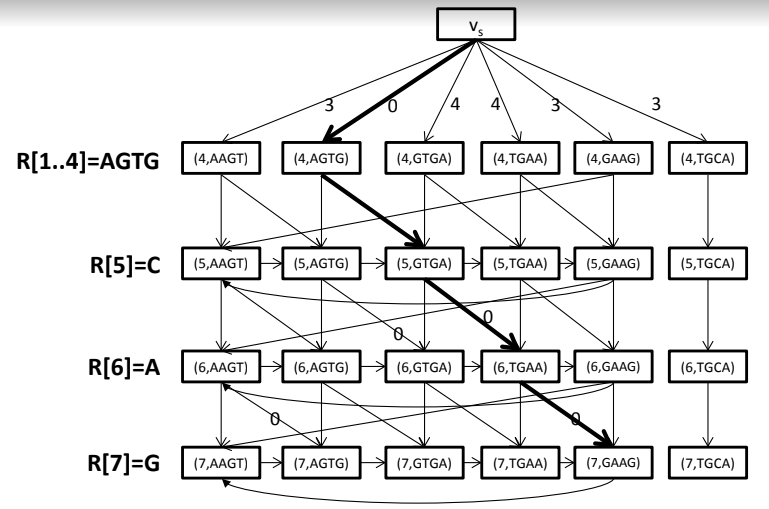
\includegraphics[width=12cm]{spectralEdit.PNG}
\caption{Razmotrimo $R = AGTGCAG$ and $T = {AAGT, AGTG, GAAG, GTGA, TGAA, TGCA}$. Ova figura pokazuje odgovarajući graf zavisnosti. Ivice za umetanje su sve horizontalne ivice. Ivice za brisanje su sve vertikalne ivice. Ivice poklapanja/nepoklapanja su sve kose ivice. Sve ivice bez oznake su težine 1. Podebljana putanja $v_s$ do $(7, GAAG)$ je najkraća putanja među svim čvorovima $(7, t)$ za $t \in T$. Težina ove putanje je 1.}
\end{figure}


%Slika algoritma spectral edit
\begin{figure}[h]
\centering
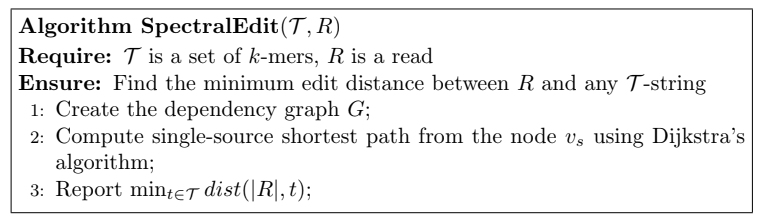
\includegraphics[width=12cm]{algoritamSpectralEdit.PNG}
\caption{SpectralEdit(T, R) algortam računa minimalno edit rastojanje između R i bilo kog $\tau$-stringa.}
\end{figure}

\section{k-mer counting}

Jedan konceptualno jednostavan, ali osnovni problem je k-mer brojanje. Ovo je jedan potprogram koji se koristi u korekciji grešaka čitanja. Takođe može biti korišćen u koraku asembliranja (Section 5.3.3), ponavljanju detekcije i kompresije genomskih podataka (Section 10.4.1). Problem je definisan na sledeći način. Ulaz je skup čitanja R i parametar k. Neka je Z skup svih mogućih k-mera (podstringovi dužine k) koji se pojavljuju u R. Naš problem je da izračunamo frekvenciju pojavljivanja k-mera u Z. U nastavku ćemo razmotriti 4 rešenja: \textbf{(1) jednostavno heširanje, (2) JellyFish, (3) BFCounter i (4) DSK.}\\

\textbf{Jednostavno heširanje}: Problem k-mer brojanja može biti rešen implementiranjem asocijativnog niza koristeći heširanje (see Section 3.4.1). Kada je k malo (npr. manje od 10), koristimo savršeno heširanje. Primetimo da svaki k-mer z može biti kodiran kao 2k-bitni binarni intidzer b(z) supstitucijom A, C, G, T u z pomoću 00, 01, 10, 11 respektivno. Tako izgrađujemo tabelu $Count[0..4^k - 1]$ veličine $4^k$ tako da svaki ulaz $Count[b(z)]$ čuva frekvenciju k-mera z u skupu Z. Preciznije,  inicijalizujemo svaki ulaz u $Count[0..4^k - 1]$ na 0. zatim, iterativno skeniramo svaki k-mer z u Z i uvećavamo $Count[b(z)]$ za 1. Na kraju, svi nenula ulazi u $Count[]$ predstavljaju pojavljivanja k-mera u Z i možemo prijaviti broj njihovih pojavljivanja. Figura 5.8(a) predstavlja primer koji ilustruje ovaj jednostavni metod prebrojavanja.\\

Pretpostavimo da je $N = |Z|$. Gore navedeni pristup je veoma efikasan. Njegovo vreme izvršavanja je $O(N + 4^k)$. Kako treba da izgradimo tabelu veličine $4^k$, prostorna složenost je $O(4^k)$. Kada je k veliko, gore navedeni algoritam ne može da radi, jer zahteva previše prostora.\\

\textbf{JellyFish}: Moguće je smanjiti veličinu heš tabele koristeći otvoreni mehanizam adresiranja (see Section 3.4.1). Neka je h() heš funkcija i $H[0..\frac{N}{\alpha} - 1]$ heš tabela koja čuva niz k-mera gde je $\alpha$ faktor opterećenja $(0 < \alpha \leq 1)$. Takođe, izgrađujemo tabelu $Count[0..\frac{N}{\alpha} - 1]$ gde $Count[i]$ čuva broj za k-mer $H[i]$.\\

Za svaki k-mer iz Z, heširamo z u neki ulaz H[i] gde je $i = h(z)$. Ako $H[i]$ nije prazan i $H[i] \neq z$, ne možemo čuvati z u $H[i]$. Ova situacija se naziva kolizija. Kolizija može biti razrešena koristeći otvoreni mehanizam adresiranja. Na primer, možemo razrešiti koliziju linearnim pokušajem. Ovim metodom pokušavamo da uvećamo indeks i za 1 kada se kolizija dogodi sve dok je $H[i] = z$ ili je ulaz $H[i]$ prazan. Funkcija hashEntry() iz Figure 5.9 ilustruje šemu linearnog pokušaja za razrešavanje kolizije. Ako $hashEntry(z, h, \frac{N}{\alpha})$ vraća prazan ulaz $H[i]$, onda z ne postoji u heš tabeli i postavljamo $H[i] = z$ i $Count[i] = 1$. U suprotnom, ako $hashEntry(z, h, \frac{N}{\alpha})$ vraća ulaz $H[i] = z$, uvećavamo $Count[i]$ za jedan. Nakon sto su svi k-meri iz Z obrađeni, prikazujemo $(H[i], Count[i])$ za sve nenula ulaze $H[i]$.\\

%Figura 5.8 i objasnjenje 
\begin{figure}[h]
\centering0
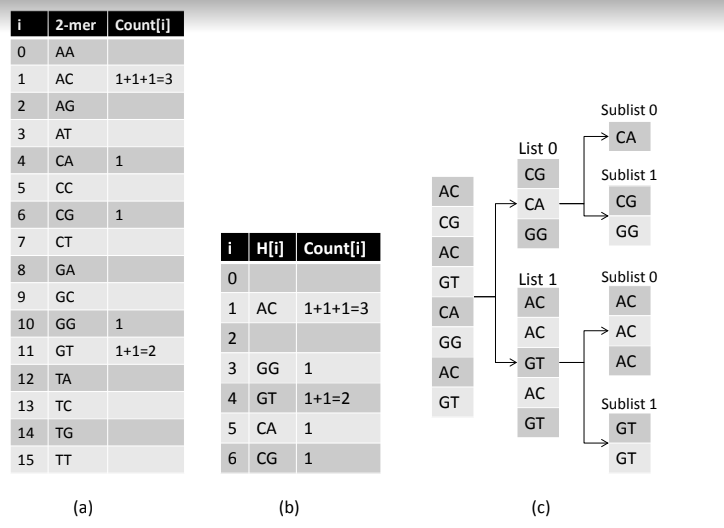
\includegraphics[width=12cm]{58_3algoritma.PNG}
\caption{Razmotrimo skup Z = \{AC, CG, AC, GT, CA, GG, AC, GT\}. (a) ilustruje jednostavan k-mer counting metod koji koristi count tabelu veličine 4^k. \(b\) ilustruje Jellyfish k-mer counting metod koji koristi heš tabelu velicine 7. Hes funkcija je $h(z) = b(z)$ mod 7. Na primer, GT se smešta na 4. mesto, jer je $h(GT) = 4$. Postoji jedna kolizija u ovom primeru. Kako je $h(CA) = 4$, CA je u koliziji sa GT. Linearnim isprobavanjem, CA se umesto na 4. mesto smešta na 5. mesto. (c) ilustruje DSK k-mer counting metod. Pretpostavljamo da je $h(z) = b(z)$, $n_{list} = 2$ i $n_{sublist} = 2$. DSK deli Z u $4(= n_{list} \cdot n_{sublist})$ podliste. Zatim se pokreće Jellyfish metod radi izračunavanja k-mera u svakoj podlisti.}
\end{figure}

% Slika algoritma
\begin{figure}[h]
\centering0
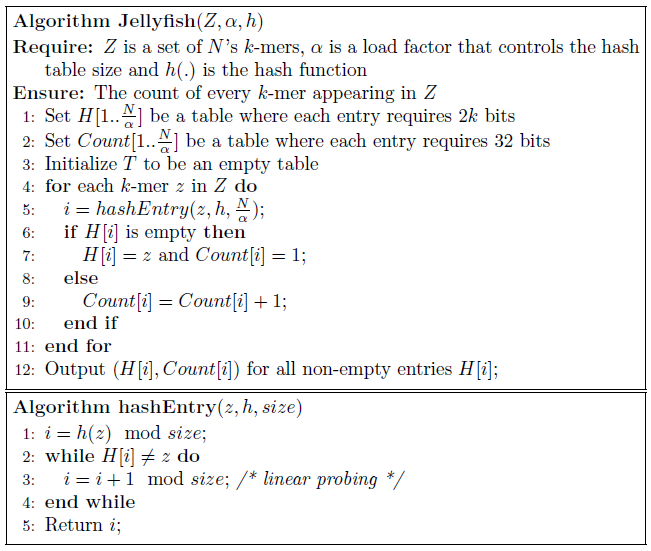
\includegraphics[width=12cm]{Jellyfish5_9.PNG}
\caption{Jellyfish algoritam za problem prebrojavanja k-mera.}
\end{figure}


Gore pomenuti algoritam je detaljnije pojašnjen na Figuri 5.9. Figura 5.8 (b) daje jedan primer koji ilustruje ovaj algoritam. On je efikasniji, ukoliko ne postoji kolizija. U praksi, očekivani broj kolizija je manji, ukoliko za opterećujući faktor važi $\alpha \leq 0.7$. Zatim, očekivano vreme izvršavanja je $O(N)$. Što se tiče prostorne složenosti, tabele $H[]$ i $Count[]$ zahtevaju $\frac{N}{\alpha}(2k + 32)$ bitova, pretpostavljajući da broj zauzima 32 bita.\\

Gore pomenuta ideja je iskorišćena u JellyFish algoritmu.\\

Iako $JellyFish$ algoritam koristi manje prostora od metode naivnog prebrojavanja, $JellyFish$ heš tabela mora biti veličine koja je jednaka bar broju jedinstvenih k-mera iz Z. $JellyFish$ i dalje zahteva mnogo memorije, kada je broj jedinstvenih k-mera u Z veliki.\\

U mnogim aplikacijama, interesuju nas samo k-meri koji se pojavljuju najmanje q puta. Ako bismo mogli da izbegnemo čuvanje k-mera koji se pojavljuju manje od q puta, sačuvali bismo mnogo memorije. Melsted et al. je predložio \textbf{BFCounter} koji prebrojava samo k-mere koji se pojavljuju najmanje q puta. On koristi counting Bloom filter da odredi da li se k-mer pojavljuje najmanje q puta. Definicija ovog filtera je u Section 3.4.3. To je prostorno efikasna struktura podataka koja nam dozvoljava da dodamo bilo koje k-mere u nju i ispitamo da li se k-mer pojavljuje najmanje q puta. Primetimo da je counting Bloom filter probabilistička struktura podataka. Iako on može dati pogrešno pozitivan (pogrešan izveštaj da k-mer postoji ili pogrešno proceniti broj k-mera), ali ne može dati pogrešno negativan rezultat. BFCounter održava counting Bloom filter B i heš tabelu H. Sastoji se od 2 faze. Prva faza počinje sa praznim counting Bloom filterom B i praznom heš tabelom H. U ovoj fazi se skeniraju k-meri iz Z jedan po jedan. Za svaki k-mer $z\inZ$ proverava se da li se z pojavljuje najmanje $q - 1$ puta u counting Bloom  filteru B utvrđivanjem da li je $countBloom(x, B) \geq q-1$. Ako nije , umećemo z u Z pomoću $insertBloom(z, B)$. U suprotnom, z se pojavljuje najmanje q puta. Proveravamo da li je z u heš tabeli H. Ako nije, umećemo z u neki prazan $H[i]$ i postavljamo $count[i] = 0$. \\

U drugoj fazi se obavlja stvarno brojanje. Vrši se skeniranje k-mera iz Z jednog po jednog. Za svaki k-mer z iz Z, ako se z pojavljuje u heširanom ulazu $H[i]$, onda uvećavamo $count[i]$ za 1. Detaljan pseudokod je prikazan na Figuri 5.10. \\

Vreme izvršavanja BFCounter algoritma je $O(n)$. Što se tiče prostorne složenosti, counting Bloom filter zahteva $O(N log(q))$. Prostor za $H[]$ i $Count[]$ je $\frac{N'}{\alpha}(2k + 32)$ bitova, gde je $N'$ broj k-mera koji se pojavlkjuju najmanje q puta. Primetimo da je $N' \leq \frac{N}{q}$. \\

\textbf{DSK}: Iako je BFCounter prostorno efikasan, njegova prostorna složenost i dalje zavisi od broja N k-mera u Z. Pretpostavimo da je memorija fiksirana tako da bude M bitova i da je memorija diska fiksirana tako da bude D bitova. Da li mozemo i dalje izračunati pojavljivanja k-mera efikasno? Rizk et al. [245] nam daje pozitivan odgovor i predlaže metod koji se naziva \textbf{DSK}. Ideja ovog metoda je da podelimo skup Z k-mera u različite liste tako da svaka lista bude smestena na disk koristeći D bitova; zatim, za svaku listu, k-meri iz liste se dalje dele u podliste tako da svaka podlista može biti sačuvana u memoriji koristeći M bitova; na kraju, frekvencije k-mera u svakoj podlisti se izračunavaju algoritmom $JellyFish$ na figuri 5.9. \\

Preciznije, k-meri u Z su podeljeni u $n_{list}$ lista približno slične dužine. Kako disk ima D bitova i svaki k-mer može biti reprezentovan u 2k bitova, svaka lista može čuvati $l_{list} =  \frac{D}{2k}$ k-mera. Kako imamo N k-mera u Z, postavljamo $n_{list} = \frac{N}{n_{list}} = \frac{2kN}{D}$. Ovo deljenje se obavlja heš funkcijom $h()$ koja ravnomerno mapira ave k-mere u $n_{list}$ lista. Preciznije, za svaki k-mer z iz Z, z se dodeljuje i-toj listi, ako je $h(z) mod n_{list} = i$. \\

Zatim, svaka lista se dalje deli u podliste, pri čemu je svaka dužine $l_sublist$. Svaka podlista će biti obrađena u memoriji pomoću algoritma JellyFish, koji zahteva $\frac{l_{sublist}}{0.7}(2k +32)$ bitova. Kako memorija ima M bitova, tako imamo $l_{sublist} = \frac{0.7M}{(2k + 32)}$. \\

%Figura 5.10
\begin{figure}[h]
\centering0
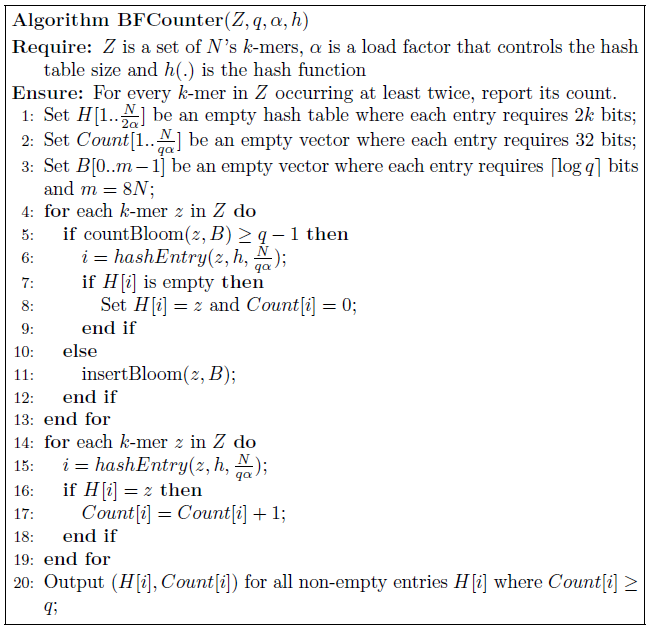
\includegraphics[width=12cm]{BFCounter5_10.PNG}
\caption{Prostorno efikasan algoritam za prebrojavanje k-mera koji broji samo k-mere koji se pojavljuju najmanje q puta.}
\end{figure}

Broj podlista je jednak $n_{sublist} = \frac{n_{list}}{n_{sublist}} = \frac{D(2k + 32)}{0.7(2k)M}$. Slično, svaka lista je podeljena u podliste heš funkcijom $h()$. Preciznije, za svaki k-mer s u i-toj listi, s je dodeljeno j-toj podlisti, ako je $(\frac{h(s)}{n_{list}}) mod n_{sublist} = j$. \\

Za svaku podlistu dužine $l_{sublist} = {0.7M}{2k + 32}$, koristeći M bitova,  brojimo broj pojavljivanja svakog k-mera u podlisti koristeći $Jellyfish(d_j, 0.7, h)$ na figuri 5.9. \\ 

Figura 5.8(c) nam daje primer za ilustraciju izvrsavanje algoritma DSK. Pretpostavimo da je $n_{list} = 2$, $n_{sublist} = 2$ and $h(z) = b(z)$ za svaki $z \in Z$. Kako je $n_{list} = 2$, algoritam izvršava 2 iteracije. Mi ovde opisujemo nultu iteraciju. (Prva iteracija se izvršava slično.) Prva faza nulte iteracije skenira sve k-mere iz Z i identifikuje svaki k-mer $z \in Z$ koji pripada nultoj listi. Na primer, $h(GG) = 10$, kako je $h(GG) mod n_{list} = 0$ i $\frac{h(z)}{n_{list}} mod n_{sublist} = 1$, GG pripada nultoj listi i prvoj podlisti. nakon toga, nulta lista se deli na nultu podlistu $\{CA\}$ i prvu podlistu $\{CG, GG\}$. Obe podliste su zapisane na disku. Druga faza čita svaku podlistu iz memorije i broji k-mere koristeći $Jellyfish$ algoritam. \\

Zapazimo da će ovaj algoritam zapisati samo jednom svaki k-mer iz Z, iako će svaki k-mer pročitati $n_{list}$ puta. Stoga, ovaj algoritam neće generisati mnogo pristupa disku radi pisanja. Zatim, analizirajmo vremensku složenost. Za i-tu iteraciju, algoritam numeriše sve k-mere u Z, što oduzima $O(n)$ vremena. Zatim, algoritam identifikuje $\frac{D}{2k}'s$ k-mera koji pripadaju i-toj listi i zapisuje ih na disk, što oduzima $O(\frac{D}{k})$ vremena. Nakon toga, algoritam  čita u $\frac{D}{2k}'s$ k-mera i izvodi brojanje, što oduzima $O(\frac{D}{k})$ vremena. Tako da svaka iteracija zahteva $O(N + \frac{D}{k}) = O(N)$ vremena, gde je $N > \frac{D}{2k}$. Kako imamo $n_{list} = \frac{2kN}{D}$ iteracija, algoritam se izvršava u $O(kN^2)$ očekivanom vremenu. Kad je $D = \theta(N)$, algoritam se izvršava u $O(kN)$ očekivanom vremenu. \\

\subsection{Base-by-base pristup proširenja}

Nakon što su sva očitavanja korigovana, mogu zalepiti korigovana čitanja kako bismo formirali podfragmente uzorka genoma, koji se nazivaju kontigzi(proveri). Postoje 2 pristupa konstrukcije kontiga: base-by-base pristup proširenja i Debrujin grafovski pristup. Ova sekcija pokriva base-by-base pristup proširenja. \\

Base-by-base pristup proširenja rekonstruiše svaki kontig tako što ga proširuje base by base. Metod počinje tako što nasumično biramo čitanje za šablon. \\

%Figure 5.11
\begin{figure}[h]
\centering
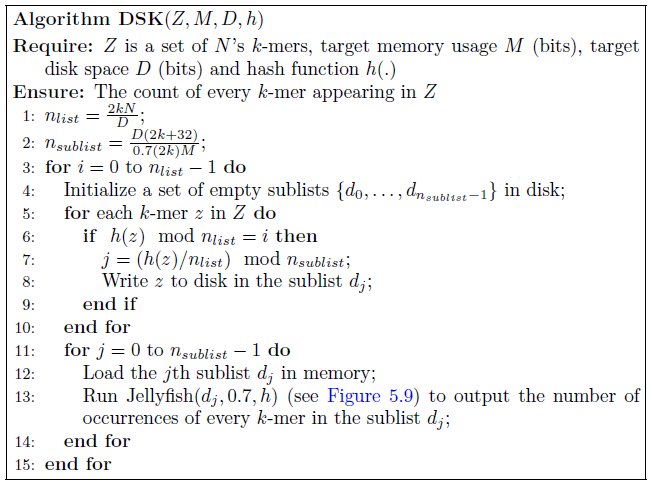
\includegraphics[width=12cm]{DSK5_11.PNG}
\caption{DSK algoritam}
\end{figure}

%Figure 5.12
\begin{figure}[h]
\centering
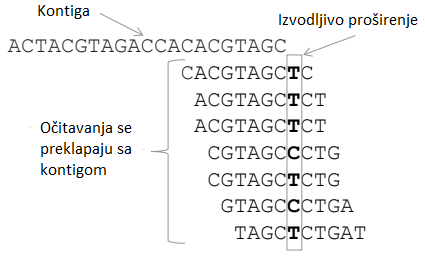
\includegraphics[width=12cm]{contig5_12.PNG}
\caption{Gornja sekvenca je šablon. Postoji T čitanja koja su poravnata na $3'$ kraju obrasca. Pravougaonik pokazuje da su baze C i T izvodljivo proširenje šablona. Kako je T konsenzus, base-by-base metoda proširenja će proširiti kontig sa bazom T.}
\end{figure}

Zatim, čitanja su poravnata na dva kraja (3' kraj i 5' kraj) šablona. Na osnovu poravnanja se dobija konsenzusna baza i obrazac se proširuje takvom bazom. Figura 5.12 ilustruje base-by-base korak proširenja. Proširivanje se ponavlja sve dok ima konsenzusa. Zatim, proširivanje prestaje i dobijamo kontig. Izvodimo proširivanje i na 3' kraju i na 5' kraju obrasca. Figura 5.13 nam daje pseudokod ovog metoda. \\

%SSAKE [309], VCAKE [117] and SHARCGS [69]
SSAKE $[309]$, VCAKE $[117]$ and SHARCGS $[69]$ su primeri metoda koji koriste ovaj pristup kako bi izgradili kontige. Iako je bazno produženje jedostavno, ono teži da daje kratke kontige zbog 2 problema. Prvi, početni šablon je nasumično izabrano očitavanje. Ako očitavanje sadrži greške sekvenciranja ili ako je u ponovljenom regionu, to će uticati na proširenje. Drugi problem se dešava kada proširimo šablon u neke ponovljene regione. Ponavljanje stvara grane i gore navedeni pristup ne može da ih razreši. \\

Da bismo rešili prvi problem, biramo očitavanje za šablon, ako je malo verovatno da ono sadrži grešku sekvenciranja ili ako je malo verovatno da će biti u ponovljenom regionu. Koristeći ideju u sekciji 5.3.1, broje se frekvencije svih k-mera svih očitavanja. Očitavanje R se bira za šablon, ako su frekvencije svih njegovih k-mera unutar nekih korisnički definisanih pragova $\theta_{min}$ i $\theta_{max}$. Ako je broj pojavljivanja nekog k-mera manji od $\theta_{min}$, R će verovatno sadržati grešku sekvenciranja. Ako je broj pojavljivanja nekog k-mera veći od $\theta_{max}$, R će se verovatno naći u ponovljenom regionu. Ova dva praga mogu biti određena proučavanjem histograma frekvencija svih k-mera ulaznih sekvenci očitavanja.\\

Za drugi problem, rešenje je korišćenje informacija o povezivanju paired-end očitavanja za rešavanje nasumičnosti. Ovaj pristup je korišćen od strane $PE-asemblera [9]$. Figura 5.14 ilustruje tu ideju. Pretpostavimo da možemo proširiti šablon koristeći 2 različita očitavanja (crno i sivo). Ne možemo odlučiti koje je ispravo (pogledati Figuru 5.14(a)). Kako svako očitavanje ima svog para, možemo biti u stanju da donesemo odluku. Postoje 2 slučaja. U prvom slučaju, ako parnjak crnom očitavanju može biti poravnat sa šablonom, možemo verovati crnom očitavanju (Figura 5.14(b)). U drugom slučaju, pretpostavimo  da postoji nekoliko očitavanja R koja su poravnata sa šablonom i parnjaci od R mogu biti poravnati sa panjakom crnog očitavanja (pogledati Figuru 5.14(c)). Onda možemo verovati i crnom očitavanju. Drugim rečima, informacije o povezanosti paired-end očitavanja mogu pomoći u  filtriranju onih lažno pozitivnih poravnanja.\\

%Figure 5.13
\begin{figure}[h]
\centering
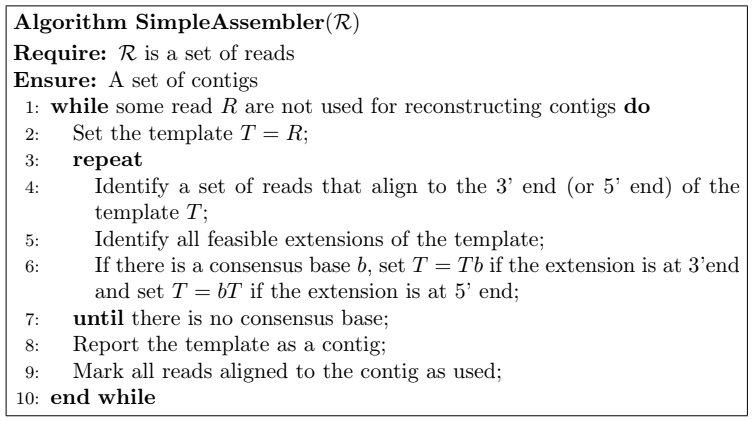
\includegraphics[width=12cm]{SimpleAsembler5_13.PNG}
\caption{Jednostavan base-by-base priširivački asembler}
\end{figure}

\subsection{Debrujin grafovski pristup}

Prethodna sekcija je pokrivala base-by-base pristup proširenja za konstruisanje kontiga. Drugi pristup je zasnovan  na Debrujinom grafu. Debrujin grafovski pristup je uveden u "Indury and Waterman [113]". Danas, ovo je glavni pristup za asembliranje kratkih očitavanja. Postojeće metode uključuju Velvet [329], SOAPdenovo [176], Euler - SR [38], IDBA[277], ABySS [275], ALLPATHS [34] i Edena [100]. \\

Prvo definišimo DeBrujinov graf. Razmotrimo skup očitavanja R i parametar k; Debrujinov graf je graf $H_k = (V, E)$, gde je V skup svih k-mera skupa R i k-meri u i v formiraju granu $(u, v) \in E$, ako su u i v prefiks dužine k i sufiks nekog podstringa iz R dužine $k + 1$, respektivno. Pretpostavljajući da je N ukupna dužina svih očitavanja iz R, Debrujinov graf može biti konstruisan u $O(N)$ vremenu.\\

Na primer, razmotrimo skup stringova $R = \{ACGC, CATC, GCA\}$. Pretpostavimo da hocemo da izgradimo Debrujinov graf za k-mere. Tada je verteks skup $\{AC, AT, CA, CG, GC, TC\}$. Figura 5.15(a) nam daje Debrujinov graf. \\

Uzorak genoma se može predvideti identifikovanjem Ojlerove putanje (Ojlerova putanja je putanja koja obilazi svaku granu grafa $H_k$ tačno jednom) grafa $H_k$. \\

%Figura 5.14(a)
\begin{figure}[h]
\centering
\includegraphics[width=12cm]{Figura5_14.PNG}
\caption{(a) Gornja sekvenca je šablon. Dva ovačitanja (crne i sive boje) se mogu poravnati sa $3'$ krajem šablona. Na osnovu crne boje očitavanja, sledeća baza je C. Na osnovu sive boje očitavanja, sledeća baza je T. Crno očitavanje je vrlo verovatno ispravno, ako se parnjak crnog očitavanja poravnjava sa šablonom (Figura (b)) ili se parnjak crnog očitavanja poravnjava sa parnjakom drugog očitavanja R koje se poravnjava sa šablonom (Figura(c)).}
\end{figure}

%Figura 5.15
\begin{figure}[h]
\centering
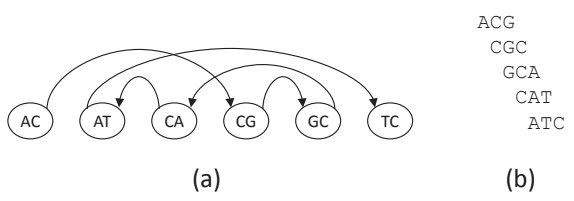
\includegraphics[width=9cm]{Figura5_15.PNG}
\caption{(a) Debrujin graf $H_3$ za $R = {ACGC, CATC, GCA}$. (b)
 Preklapanje 5 3-mera koji odgovaraju 5 ivicama od $H_3$.}
 \end{figure}

%Figura 5.16
\begin{figure}[h]
\centering
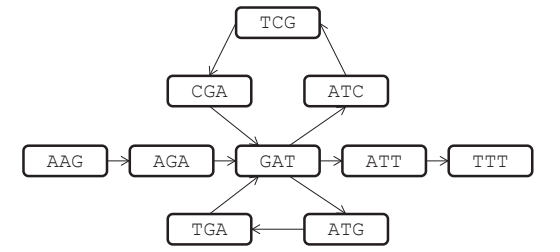
\includegraphics[width=9cm]{Figura5_16.PNG}
\caption{Debrujin graf $H_3$ za $R = \{AAGATC, GATCGAT, CGATGA, ATGATT, GATTT\}$ }
\end{figure}


Primetimo da Ojlerova putanja grafa $H_k$ može biti izračunata u $O(n)$ vremenu, ako $H_k$ ima n grana. Na primer, na Figuri 5.15(a) postoji jedinstvena putanja od čvora AC do čvora TC. Preklapanjem svih 3-mera ivica u redosledu putanje (pogledati Figuru 5.15(b)) dobijamo sekvencu $ACGCATC$. Sekvenca $ACGCATC$ je zapravo superstring formiran preklapanjem čitanja $ACGC, GCA, CATC$ u redu. Ovaj primer sugeriše da genom može biti dobijen na osnovu Debrujinovog grafa od R.\\

Medjutim, Ojlerova putanja ne može biti jedinstvena u $H_k$. Na primer, razmotrimo skup čitanja $R = \{AAGATC, GATCGAT, CGATGA, ATGATT, GATTT\}$. Pretpostavimo da je $k = 3$.\\

Debrujinov graf $H_3$ je prikazan na Figuri 5.16. Postoje 2 Ojlerove putanje u $H_3$. Ako prvo obiđemo gornji ciklus, dobijamo $AAGATCGATGATTT$. Ako prvo obiđemo donji ciklus, dobijamo $AAGATGATCGATTT$. \\

Ovaj primer ukazuje da Ojlerova putanja mozda neće vratiti ispravnu sekvencu. Čak još gore, Ojlerova putanja možda neće postojati u nekom grafu $H_k$. \\

U daljem tekstu opisujemo Debrujinov grafoovski asembler kada (1) ne postoji greška sekvenciranja i (2) postoji greška sekvenciranja.
Zatim ćemo razmatrati pitanje odabira k. \\

\subsection{Debrujinov asembler (bez greške skvenciranja)}

Kako Ojlerova putanja nije jedinstvena i možda ne postoji, ne težimo tome da dođemo do kompletnog genoma. Umesto toga, pokušavamo da dobijemo skup kontiga. Kontig je maksimalna jednostavna putanja u $H_k$. Preciznije, svaka maksimalna putanja je maksimalna putanja u $H_k$ tako da svaki čvor (osim početnog i krajnjeg) ima unutrašnji stepen 1 i spoljašnji stepen 1. Figura 5.17 nam daje pseudokod ovog jednostavnog metoda.\\

Za Debrujinov graf $H_3$ na Figuri 5.16 možemo konstruisati 4 kontiga: $AAGAT, GATCGAT, GATGAT, GATTT$. Primetimo da je k veoma važan parametar. Dobijamo različite skupove kontiga, ukoliko menjamo k. Kako bismo ilustrovali ovaj problem, Figura 5.18 daje Debrujinov graf za $k = 4$ i $k = 5$.\\

%Algoritam Debrujin asembler
%Figura 5.17
\begin{figure}[h]
\centering
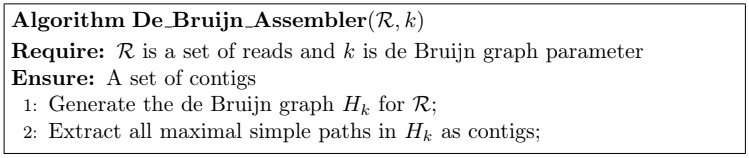
\includegraphics[width=9cm]{Figura5_17.PNG}
\caption{Jednstavan Debrujinov grafovski asmbler.}
\end{figure}

%Figura 5.18
\begin{figure}[h]
\centering
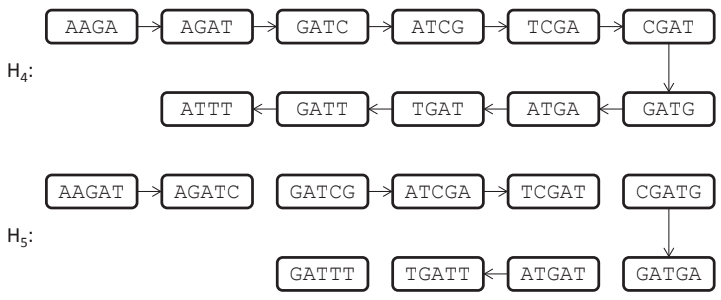
\includegraphics[width=9cm]{Figura5_18.PNG}
\caption{Debrujinov graf $H_4$ i $H_5$ za $R = {AAGATC, GATCGAT, CGATGA, ATGATT, GATTT}$}
\end{figure}

Kada je $k = 4$, $H_4$ je prosta putanja. Možemo konstruisati jedan kontig $AAGATCGATGATTT$.\\

Kada je $k = 5$, $H_5$ sadrži 5 povezanih komponenata i svaka je prosta putanja.\\

Možemo konstruisati 5 kontiga: $AAGATC, GATCGAT, CGATGA, ATGATT, GATTT$. \\

Iz gore navedenih primera, primećujemo da je Debrujinov graf dobar kada znamo ispravno k. Kada je k malo (pogledati $H_3$ na Figuri 5.16), postoje mnoge grane zbog ponovljenih regiona. Ovo rezultuje mnogim kratkim kontizima. Kada je k veliko (pogledati $H_5$ na Figuri 5.18), neki k-meri nedostaju (naročito za regione sa velikom pokrivenošću). Ovo rezultuje nepovezanim komponentama, koje takođe generišu mnoge kratke kontige. Moramo identifikovati k kako bi se pronašla ravnoteža između ova dva pitanja. Više ćemo razgovarati o izboru parametra k u sekciji 5.3.3.3 \\

\subsection{Debrujinov graf (sa greškama sekvenciranja)}

Prethodna podsekcija pretpostavlja da nema grešaka sekvenciranja u očitavanjima, što je nerealno. Kada postoje greške u sekvenciranju, možemo pokušati da ih uklonimo iz Debrujinovog grafa. Ova sekcija predstavlja rešenje koje su predložili Žerbino i Birnei. Obratimo pažnju da kratka očitavanja imaju nisku stopu pogreške (1 greška na svakih 100 baza). Većina k-mera sadrži najviše 1 grešku. Ovi pogrešni k-meri će kreirati 2 moguća anomalna podgrafa u Debrujinovom grafu: vrh (špic) i mehur. U nastavku ćemo opisati kako da ih sredimo.\\

%Figure 5.19
\begin{figure}[h]
\centering
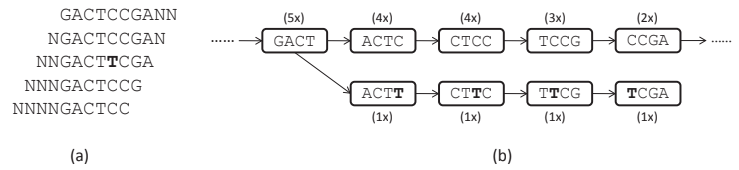
\includegraphics[width=9cm]{Figura5_19.PNG}
\caption{(a) je višestruko poravnanje skupa od 5 čitanja, gde treće čitanje ima grešku sekvenciranja (prikazana podebljanim fontom). (b) prikazuje Debrujinov graf koji odgovara skupu čitanja iz (a). Vrh je napravljen. Brojevi u zagradama označavaju mnogostrukost 4-mera.}
\end{figure}

Vrh je put dužine najviše k gde svi unutrašnji čvorovi imaju ulazni stepen 1 i izlazni stepen 1, dok jedan od njegovih krajeva ima ulazni ili izlazni stepen 1. To može proizvesti potencijalni kontig  dužine najviše 2k. Figura 5.19 ilustruje vrh kreiran na osnovu jednog nepoklapanja u jednom čitanju. Ako svi čvorovi na vrhu niske mnogostrukosti (manji broj k-mera), takav kratak kontig teško da može biti istinit. Možemo ukloniti ovaj vrh iz Debrujinovog grafa. Primetimo da uklanjanje vrha iz Debrujinovog grafa može generisati jos vrhova. Procedura mora uklanjati vrhove rekurzivno. \\

Mehurići su 2 staze koje počinju od istog verteksa i završavaju se u istom verteksu, gde 2 staze predstavljaju različite kontige koji se razlikuju samo po jednom nukleotidu. Na primer, Figura 5.20 (a) sadrži skup očitavanja gde treće čitanje ima jedno nepoklapanje. Figura 5.20 (b) prikazuje odgovarajući Debrujinov graf i jedan mehur koji se formira. Gornja putanja mehura predstavlja $GACTCCGAG$. Donja putanja mehura predstavlja $GACTTCGAG$. Kada su dve putanje u mehuru veoma slične, putanja sa nižom mnogostukošću će verovatno biti lažno pozitivna. Možemo pokušati da spojimo mehur. U primeru, 2 putanje imaju samo jedno nepoklapanje. Nadalje, budući da čvorovi u donjoj putanji imaju nižu mnogostrukost, spajamo mehur i dobijamo graf na Figuri 5.20 (c). Preciznije, možemo definisati težinu putanje $w_1 \rightarrow w_2 \rightarrow ... \rightarrow w_p$ kao $\sum_{i=1}^{p} f(w_i)$, gde je $f(w_i)$ mnogostrukost od $w_i$. Onda, kada spojimo 2 putanje u mehur, zadržaćemo putanju sa najvećom težinom. \\

Da bismo spojili mehurice, možemo koristiti algoritam turneje. Ovaj algoritam je nalik na Dijkstrinu pretragu u širinu baziranu na BFS metodu. Algoritam počinje od proizvoljnog čvora s i posećuje čvorove u rastućem poretku rastojanja od početnog čvora. Kada algoritam obrađuje neposećeni čvor u, on proverava svu njegovu decu v. Za svako dete v se izvode 2 koraka. Prvo, dodeljuje se u kao roditelj od v u BFS stablu postavljanjem $\pi (v) = u$. Drugo, ako je dete v od u posećeno, mehur je detektovan; algoritam izračunava najnižeg zajedničkog pretka c od u i v u BFS stablu definisanog sa $\pi ()$. Zatim, 2 putanje $c \rightarrow u$ i $c \rightarrow v$ se upoređuju. Ako su dovoljno slične (sa sličnošću od najmanje $80\%$ u Velvetu), spajaju se  i zadržavamo putanju sa najvećom težinom putanje. Algoritam je detaljnije prikazan na Figuri 5.21.\\

%Figura 5.20
\begin{figure}[h]
\centering
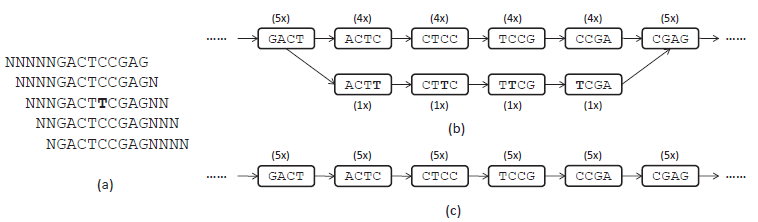
\includegraphics[width=9cm]{Figura5_20.PNG}
\caption{(a) je višestruko poravnanje skupa od 5 čitanja, gde treće čitanje ima grešku sekvenciranja (prikazana podebljanim fontom). (b) prikazuje Debrujinov graf koji odgovara skupu čitanja iz (a). Mehur je napravljen. (c) je putanja dobijena spajanjem mehurića iz (b).}
\end{figure}

Figura 5.22 ilustruje korake algoritma turneje. Originalni Debrujin graf je prikazan na Figuri 5.22 (a). Počevši od čvora r, BFS traversal se izvodi kako bi se posetili svi potomci od r u rastućem poretku rastojanja od r. BFS traversal se zaustavlja kada dođe do posećivanja već posećenog čvora. Figura 5.22 (b) prikazuje BFS stablo (podebljano) kada je čvor v ponovo posećen od strane čvora u. Identifikovanjem najnižeg zajedničkog pretka c u BFS stablu, pronalazimo 2 putanje $c \rightarrow u$ i $c \rightarrow v$ koje formiraju mehur. Spajamo 2 putanje i zadržavamo putanju sa većom mnogostrukošću. Nakon formiranja mehura, dobijamo sliku 5.22(c). Zatim se BFS nastavlja. Nakon što BFS poseti $u'$, ponovo posećuje $v'$. $c'$ je najniži zajednički predak od $u'$ i $v'$. Pronalazimo 2 putanje $c' \rightarrow u'$ i $c' \rightarrow v'$ koje formiraju mehur. Nakom formiranja mehura, dobijamo figuru 5.22(d). Zatim, ne možemo pronaći nijedan mehur i algoritam turneje se završava. \\

Nakon što uklonimo vrhove i spojimo mehuriće u Debrujinovom grafu, možemo dalje filtrirati buku uklanjanjem k-mera sa mnogostrukošću manjom ili jednakom nekom pragu m (recimo $m = 1$). Na primer na Figuri 5.22(d), ako je $m = 1$, moramo da uklonimo 2 ivice težine 1. Primetimo da se ova tehnika takođe koristi kada vršimo korigovanje greške u sekciji 5.3.1. Ukratko, ovaj odeljak predstavlja 3 trika: (1) uklanjanje vrhova, (2) spajanje mehurića i (3) filtriranje k-mera sa niskom mnogostrukošću. Kombinovanjem ovih tehnika, dobijamo algoritam koji može da obradi greške sekvenciranja i prikazan je na Figuri 5.23. \\

\subsection{Kako izabrati k?}

Kao što je objašnjeno u odeljku 5.3.3.1, odabir broja k može uticati na performanse Debrujinovog algoritma.\\

Jednostavno rešenje je pokretanje algoritma sa Figure 5.23 za višestruke k. \\

%Figure 5.21
\begin{figure}[h]
\centering
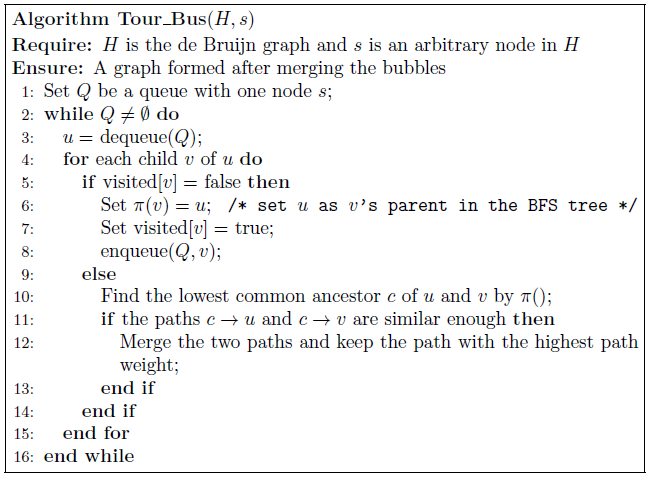
\includegraphics[width=9cm]{Figura5_21.PNG}
\caption{Algoritam turneje autobusom}
\end{figure}

Zatim se kontizi grupišu i spajaju. Ovu tehniku koriste neki transkriptorni asembleri$[193, 291]$ . \\

Jedan od problema sa ovim jednostavvnim rešenjem je taj što kontizi dobijeni različitim k imaju drugačiji kvalitet. Za kontige dobijene od $H_k$ gde je k malo, oni su veoma tačno; međutim, kontizi su kratki, jer postoji mnogo grana zbog ponavljenih regiona. Za kontige dobijene od $H_k$ gde je k veliko, oni su veći; međutim, oni mogu sadržati mnogo grešaka.\\

IDBA $[227]$ sugeiše da ne traba da gradimo Debrujinov graf nezavisno za različite k. Umesto toga, IDBA gradi Debrujinov graf $H_k$ postepeno krećući od malih k ka velikim k. Kada je k malo, možemo dobiti visokokvalitetne kontige, iako su kratki. Zatim se ovi kontizi koriste za ispravljanje grešaka u čitanjima. Postepeno, izgradjujemo Debrujinov graf $H_k$  za veće k. Kako su čitanja u R korigovana, buka (noise) u $H_k$ je redukovana. Ovo nam omogućava  da dobijemo dugačke kontige viskog kvaliteta iz $H_k$ kada je k veliko. Figura 5.24 opisuje ideju koju je predložio IDBA. \\

%Figure 5.22
\begin{figure}[h]
\centering
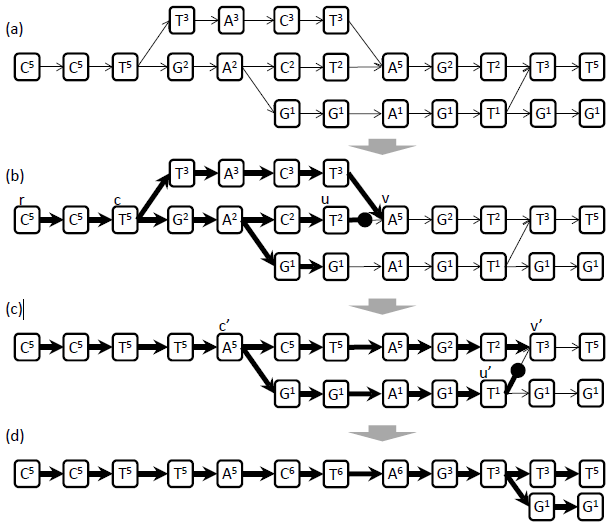
\includegraphics[width=9cm]{Figura5_22.PNG}
\caption{Ovaj primer ilustruje kako algoritam turneje autobusom (prunes)obilazi Debrujinov graf. Radi jasnoće, svaki čvor pokaztuje poslednju bazu svojih k-mera i odgovarajući celokupni stepen je njegova mnogostrukost. Algoritam izvodi pretragu u dobinu (BFS) i BFS stablo je prikazano podebljanim ivicama. Na (a) postoje 2 (ugnježdena) mehura. Na (b) iyvodimo BFS počevši od r. Kada posetimo u, dete v od u je posećeno (npr. unutar BFS stabla). Identifikujemo mehurić i spajamo ga. Zatim, dobijamo (c). Na (c) nastavljamo izvođenje BFS algoritma. Kada posetimo $u'$, dete $v'$ od $u'$ je pose'eno. Identifikujemo drugi mehur i spajamo ga. Zatim, dobijamo (d). Na (d) nastavljamo izvođenje BFS algoritma. Kako ne možemo da identifikujemo više nijedan mehurić, algoritam se završava.}
\end{figure}

%Preskoceno additional issuses


\subsection{Scaffolding}

Korak izgradnje kotiga u sekciji 5.3.2 i 5.3.3 izveštava o nizu kontiga. \\

Sledeće pitanje je kako povratiti ispravan redosled i korigovati orijentaciju kontiga u uzorku genoma. Na ovo pitanje može se odgovoriti rešavanjem scaffolding problema. Figura 5.25 daje primer skeleta za 4 kontiga A, B, C i D. Skelet je $(A, -B, -C, D)$. Primetimo da je orijentacija kontiga B i C obrnuta. Kako bismo potrvrdili skelu, možemo iskoristiti paired-end čitanja izvučena iz uzorka genoma. Setimo se u celosti sekvenciranja genoma, za svako  paired-end čitanje (na primer, čitanje i njegov par) se očekuje da se mapira u unutrašnjoj orijentaciji (zasnovano na illumina sekvenciranju) i da ima svoju veličinu umetka sa malim dometom ($span_{min}$, $span_{max}$). Paired-end čitanje treba da podržava skelet, ako je paired-end čitanje poravnato prema unutrašnjosti skele i njegova veličina umetka ne krši opseg ($span_{min}$, $span_{max}$). U ovom slučaju, za paired-end čitanje se kaže da je usklađeno. U suprotnom, ono je neusklađeno. Na primer, na Figuri 5.25, paired-end čitanje (1) ima ispravnu veličinu umetka i ispravnu orijentaciju. Tako da paired-end čitanje (1) se naziva usklađeno. Paired-end čitanja (2) i (3) imaju ispravnu veličinu umetka. Međutim, njihove orijentacije nisu ispravne. Za paired-end čitanje (4), iako ima ispravnu orijentaciju, veličina umetka je prevelika. Stoga, paired-end čitanja (2), (3) i (4) su neusklađena.\\

Problem skele je definisan na sledeći način. Ulaz je skup pair-end čitanja E i skup kontiga C. Problem skele teži da generiše orijentacije i redosled kontiga tako da broj neusklađenih čitanja bude minimalan. Figura 5.26 daje primer. Ulaz se sastoji od 3 kontiga A, B i C i od skupa paired-end čitanja koja su mapirana sa kontizima. Ako popravimo skelu kao $(A, B, C)$, sva paired-end čitanja su neusklađena. Da bismo minimizovali broj neusklađenih čitanja, skela treba da bude $(C, -B, A)$. U ovom slučaju, postoji samo jedno neusklađeno čitanje. Stoga, problem skele teži da skela bude $(C, -B, A)$.\\

%Figura 5.26
\begin{figure}[h]
\centering
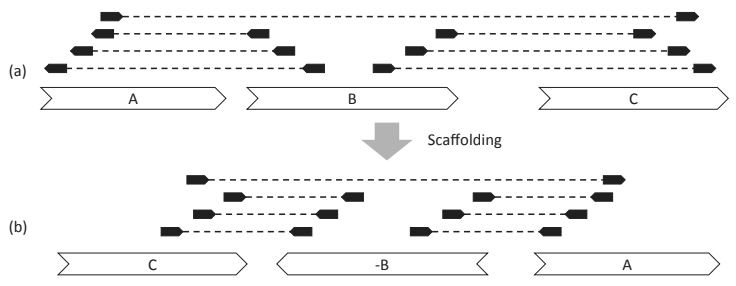
\includegraphics[width=9cm]{Figura5_26.PNG}
\caption{Primer skeleta. Ulaz čine 3 kontiga A, B i C i skup uparenih krajeva čitanja mapiranih na kontizima. Problem skeleta teži da rearanžira kontige u $(A, -B, C)$ tako da broj neslaganja čitanja bude minimalan.}
\end{figure}

Problem skele izgleda jednostavno. Huston $[111]$ je pokazao da je problem skele NP-kompletan. Čak i samo za određivanje ispravne orijentacije kontiga (na primer, nema potrebe odrediti njihove redoslede), Kececioglu i Myers $[133]$ su pokazali da je i dalje NP-kompletan. \\

Budući da je problem skele težak za izračunavanje, predložen je određen broj heuističkih ili aproksimativnih algoritama. Mnogi od njih su unutrašnje rutine kod nekih asemblerima. Neki primeri uključuju, PEAssembler $[9]$, SSAKE $[309]$, ABySS $[275]$ i SOAPenovo $[176]$. Postoje neki samostalne skele u koje uključujemo Bambus $[235]$, SSPACE $[24]$, SOPRA $[61]$, MIP Scaffolder $[258]$, Opera $[85]$, Opera-LG $[84]$ i SCARPA $[70]$. \\

Problem skele može biti rešen u 3 koraka:
\begin{enumerate}
    \item {Razgraničiti regione koji se ponavljaju unutar asembliranih kontiga.}
    \item {Izgraditi grafik.}
    \item {Identifikovati linearni redosled kontiga koji minimizuje broj neusklađenih ivica.}
\end{enumerate}

\textbf{Korak 1}: Razgraničite sve ponovljene regione unutar asembliranih kontiga. Ovaj korak poravnava sva paired-end čitanja iz E na kontige u C. Pretpostavlja se da će srednja gustina čitanja biti očekivana pokrivenost čitanja u genomu. Svaki region sa gustinom čitanja većom 1,5 puta od srednje se smatra ponovljenim regionom. Razgraničite sve ponovljene regione unutar kontiga.\\

\textbf{Korak 2}: Izgradite kontig graf. Ovaj korak definiše kontig graf. Svako paired-end čitanje $PE$ iz $\epsilon$, odbacuje se, ako se (1) oba čitanja od $PE$ poravnaju konkordantno na istom kontigu ili (2) bilo koje čitanje od $PE$ ne uspeva da se poravna na bilo kom kontigu ili se (3) bilo koje čitanje od $PE$ poravna na ponovljenom reginonu (pogledati Figuru 5.27). Svako paired-end čitanje iz E je predstavljeno kao uredjena četvorka $(X, Z, x, z)$ gde su X i Z neki orijentisani kontizi iz C i x i z su dužine kontiga X i Z, respektivno, pokrivena paired-end čitanjem. Na primer na Figuri 5.28, paired-end čitanja $PE_1$ i $PE_2$ su predstavljena kao $(A, -D, a, e)$ i $(-C, -d, d, e + f)$, respektivno.\\

\textbf{Korak 3}: Identifikujte linearni poredak kontiga koji minimizuje broj neusklađenih ivica. Ovaj korak orijentiše  i uredjuje kontige iz C kako bi se minimizovao broj neusklađenih čitanja. Ovaj problem je poznat kao problem konstrukcije skela koji je definisan na sledeći način. Ulaz je kontig graf $(C, E)$ gde je C skup kontiga, a E je skup paired-end čitanja.  Izlaz je skelet koji je definisam kao linearno uređenje kontiga iz C. Paired-end čitanje je neusklađeno, ako nije unutrašnje i njegova veličina umetka je veća od $span_{max}$. Na primer, na Figuri 5.28, paired-end čitanje $PE_2$ je neusklađeno, ako je $d + e + f > span_{max}$. Ovaj problem teži da pronađe skelet S od C koji minimizuje broj neusklađenih paired-end čitanja. \\

Ovde ćemo predstaviti greedy algoritam $[9]$. Za bilo koji skelet S koji sadrži podskup kontiga iz C definisan je skor $score(S)$ koji predstavlja ukupan broj konkordantnih paired-end čitanja umanjen za ukupan broj neusklađenih paired-end čitanja koja su poravnata na S. Greedy algoritam počinje odabirom slučajnog kontiga kao početnog skeleta S. Proces zatim proširuje skelu S nekim kontigom C (označeno kao $S \cdot C$ ili $C \cdot S$ u zavisnosti da li je C levo ili desno od S) iterativno sve dok S više ne može biti proširen. Kaže se da je kontig C desni (ili levi) izvedeni sused od S, ako S može biti proširen do $S \cdot C$ (ili $C \cdot S$) tako da postoji neko skladno paired-end čitanje čiji je jedan kraj poravnat sa S i drugi kraj poravnat sa C. Neka su $C_1, ..., C_r$ svi desni izvedeni susedi od S i neka su $C'_1, ..., C'_{r'}$ sve levi izvedeni susedi od S. Među svim mogućim permutacijama desnih izvedenih suseda od S, identifikujemo permutaciju $C_{i_1}, ... C_{i_r}$ koja maksimizuje skor $s_R = score(S \cdot C_{i_1} \cdot ... \cdot C_{i_r})$. Slično, identifikujemo permutaciju $C'_{j_1},...,C'_{j_{r'}}$ koja maksimizuje skor $s_L = score(C'_{j_1} \cdot ... \cdot C'_{j_{r'}} \cdot S)$. Ako je $s_R > \max{0, s_L}$, proširujemo S do $S \cdot C_{i_1}$. U suprotnom, ako je $s_L > \max{0, s_R}$, proširujemo S do $C_{j_{r'} \cdot S$. Ovaj proces se ponavlja sve dok ne dođemo do toga da se nijedan kraj ne može proširiti; zatim, dobijamo jednu skelu. Nakon što je dobijena skela, cela procedura se ponavlja na neiskorišćenim kontizima kako bi se identifikovale druge skele. Detaljan pseudokod  je prikazan na Figuri 5.29.  \\

%Figure 5.29
\begin{figure}[h]
\centering
\includegraphics[width=9cm]{Figura5_29.PNG}
\caption{GreedyScaffolding algoritam.}
\end{figure}

\subsection{Popunjavanje praznina}

Pomoću skela identifikujemo susedne kotige. Region između 2 susedna kotiga naziva se praznina. Za neke praznine ćemo možda moći da rekonstruišemo DNA sekvencu koristeći lokalno asembliranje. U nastavku ćemo diskutovati o jednom mogućem načinu za popunjavanje praznina.\\

%Figura 5.30
\begin{figure}[h]
\centering
\includegraphics[width=9cm]{Figura5_30.PNG}
\caption{Pretpostavimo da su kontizi A i B susedni. Ova figura pokazuje sve uparene krajeve čitanja gde se jedno od čitanja mapira na kontig A ili B, ali njegov par ne može biti da se proavna ispravno. Skupljanjem ovih čitanja možemo rekonstruisati prazninu koristeći lokalno asembliranje. (Primetimo da ova praznina ne može biti rekonstruisana korišćenjem uparenih krajeva čitanja poravnatih samo na A (siva boja) ili samo na B (crna boja). Štaviše, praznina se može sastaviti, ako koristimo sve uparene krajeve čitanja poravnate i na A i na B.) }
\end{figure}
Suppose contigs A and B are adjacent. This figure shows
all paired-end reads where one of the reads maps on contig A or B, but its
mate cannot align properly. By collecting these reads, we may reconstruct
the gap using local assembly. (Note that this gap cannot be reconstructed
using paired-end reads aligned on A only (gray color) or B only (black color).
Moreover, the gap can be assembled if we use all paired-end reads aligned on
both A and B.)

Neka su A i B susedni kontizi. Sva paired-end čitanja koja mogu biti poravnata sa desnim krajem od A ili sa levim krajem od B su izdvojena (Figure 5.30). Asembliramo ova paired-end čitanja koristeći asembler, kao SSAKE $[309]$, koji može raditi i u slučaju male pokrivenosti. Ovaj pristup nam omogućava da popunimo neke praznine ili da redukujemo veličinu nekih praznina. \\





















\newpage
\begin{thebibliography}{10}

\bibitem{A1} {{ЗОРАН ЛУЧИЋ} {\it Еуклидска и хиперболичка геометрија}, {\Lat Total design} и Математички факултет, Београд, 1997. год.}

\bibitem{A2} {{Г. КАЛАЈЏИЋ, М. ЂОРИЋ} {\it Скрипта из основа геометрије}, Математички факултет, Београд, 2002. год.}

\bibitem{A3}{{МИЛОШ РАДОЈЧИЋ} {\it Елементарна геометрија основе и елементи еуклидске геометрије}, Научна књига, Београд, 1961. год. }

\bibitem{A3}{{ЕУКЛИД} {\it Елементи}, Научна књига, Београд, 1957.год. }

\end{thebibliography}
\end{document}
